
\section{Bounds}
\label{sec:bounds}

\subsection{Patching}

Any two unimodular triangulations of $P_{m,n_1}$ and $P_{m,n_2}$ can
be patched to a unimodular triangulation of $P_{m,n_1+n_2}$. Thus we
have the follwing supermultiplicativity relation, where $\firreg(m,n)$
denotes the number of irregular unimodular triangulations of $P_{m,n}$. 

\begin{lemma}
  \label{lem:supermul}
  For $m,n_1,n_2\geq 1$ the following relations hold.
  \begin{enumerate}
    \item[\rm(i)] \mbox{\centerline{$f(m,n_1+n_2)\ge f(m,n_1)f(m,n_2)$}}
    \item[\rm(ii)] \mbox{\centerline{$\firreg(m,n_1+n_2)\ge f(m,n_1)\firreg(m,n_2)$}}
  \end{enumerate}
\end{lemma}

With respect to regular triangulations, patching is dangerous, as
demonstrated by the following example of a non-regular triangulation
of $P_{4,4}$ composed of four regular triangulations of $P_{2,2}$
(suggested by Francisco Santos).
\[
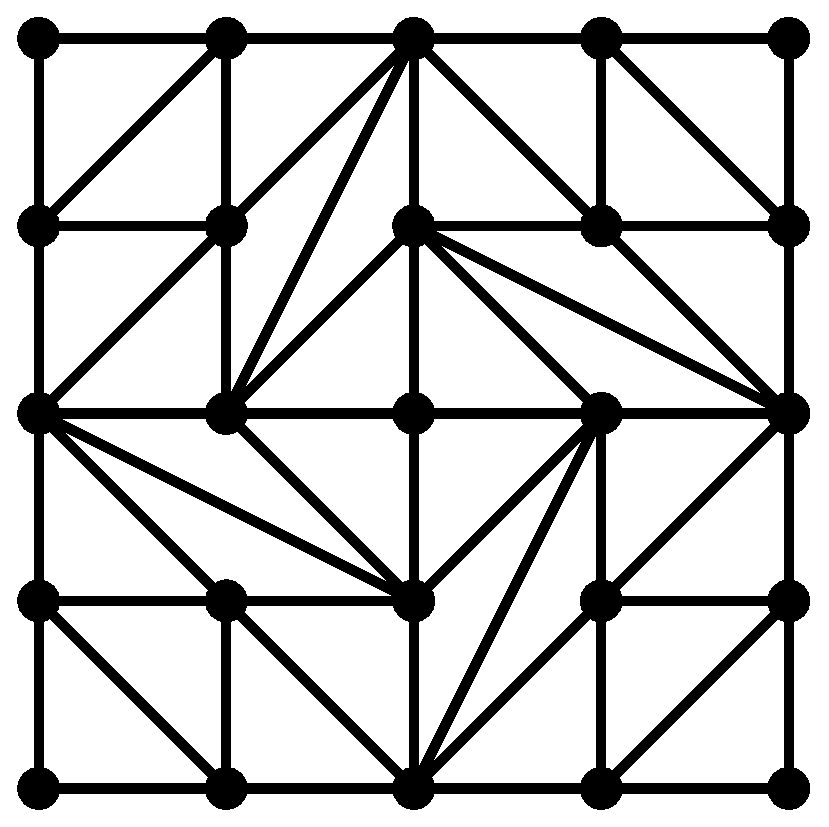
\includegraphics[height=33mm]{santos1.eps}
\]
However, a much more general theorem by Goodman and Pach
\cite{GoodmanPach} says that any two regular
triangulations of two disjoint convex polytopes $P_1,P_2\subset\R^d$
can be extended to a regular triangulation of $\conv(P_1\cup P_2)$
without additional vertices. Thus also for the regular case 
we get a (slightly weaker) supermultiplicativity relation.

\begin{lemma}
  \label{lem:supermulreg}
  For $m,n_1,n_2\geq 1$  we have
  $$
  \freg(m,n_1+n_2+1)\ge \freg(m,n_1)\freg(m,n_2)\ .
  $$
\end{lemma}

The following figure illustrates the patching of
Lemma~\ref{lem:supermulreg}:
\begin{center}
  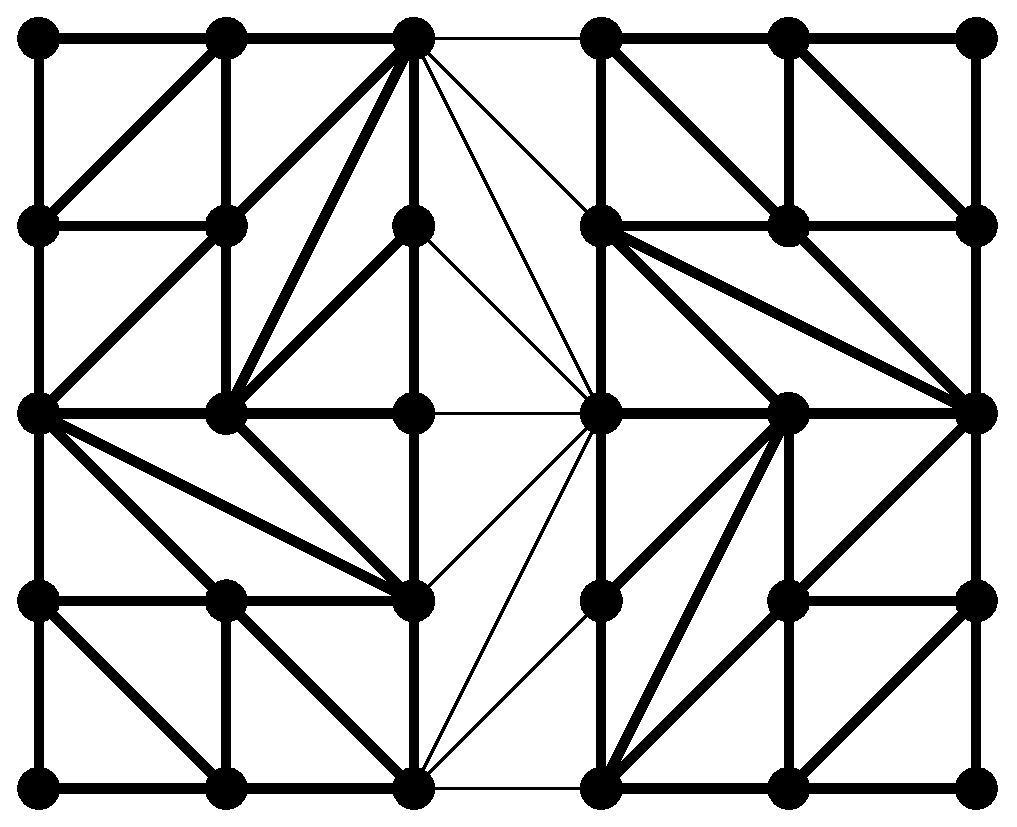
\includegraphics[height=33mm]{santos2.eps}
\end{center}

For $n_2=1$ we will (Lemma~\ref{lem:patchreg1strip}) strengthen the
inequality in Lemma~\ref{lem:supermulreg}.  

Let us fix some notations first.  For any function
$h:P_{m,n}\longrightarrow\R$ we denote by
$H:P_{m,n}\longrightarrow\R^3$ the function with
$H(x,y)=(x,y,h(x,y))$. The function~$h$ is called a \emph{lifting
  function} of a triangulation~$\mathcal{T}$ of~$P_{m,n}$, if
$\mathcal{T}$ is the image of the set of ``lower facets'' of the
$3$-polytope $\conv\{H(x,y):(x,y)\in P_{m,n}\}$ under orthogonal
projection to the $x,y$-plane (deletion of the third coordinate).

A function~$h$ is a lifting function of~$\mathcal{T}$ if and only
if~$h$ is convex and piecewise linear, and its (maximal) domains of
linearity are the triangles in~$\mathcal{T}$. In particular, one may
add to~$h$ any convex piecewise linear function whose domains of linearity
are unions of triangles of~$\mathcal{T}$ in order to obtain another
lifting function for~$\mathcal{T}$.

A triangulation is regular if and only if it has a lifting function.

The following result shows that all unimodular triangulations of a
strip of width $1$ are regular; moreover one has a lot of freedom in
choosing the respective lifting functions, which we will exploit
below.

\begin{lemma}
  \label{lem:stripreg}
  Let $\mathcal{T}$ be a unimodular triangulation of a lattice
  trapezoid with two parallel vertical or horizontal sides $S_0$ and
  $S_1$ at distance one. Every piecewise linear function
  $h_0:S_0\longrightarrow\R$ that is strictly convex on $S_0\cap\Z^2$
  can be extended to a lifting function for~$\mathcal{T}$.
\end{lemma}

\begin{proof}
  Let $p_0,\dots,p_r$ be the integral points on $S_0$, and let
  $\{e_{i,1},\dots,e_{i,k(i)}\}$ be the edges of $\mathcal{T}$
  connecting $p_i$ to $S_1$. Let $S_0^+(i)$ and $S_0^-(i)$ be the
  closures of the two components of $S_0\setminus\{p_i\}$. Then we may
  decompose the function $h_0$ as
  $$
  h_0(x)=\sum_{i=0}^r\sum_{j=1}^{k(i)}h_{i,j}(x)\ ,
  $$
  where each $h_{i,j}$ is a convex function on $S_0$, linear both
  on $S_0^+(i)$ and on~$S_0^-(i)$, and having its  unique break-point
  at~$p_i$.

  Now we extend each $h_{i,j}$ to a convex, piecewise-linear function
  defined on the entire trapezoid such that
  it has a break-line at the edge $e_{i,j}$ and is linear above
  and below this line.
  Then the sum of all $h_{i,j}$ is a lifting function for~$\mathcal{T}$.
\end{proof}


\begin{prop}
\label{prop:fregm12}
  For $n\geq 1$ the following relations hold.
  \begin{enumerate}
  \item[\rm(i)] \mbox{\centerline{$\freg(1,n)=f(1,n)=\binom{2n}{n}$}}
  \item[\rm(ii)] \mbox{\centerline{$\freg(2,n)=f(2,n)$}}
  \end{enumerate}
\end{prop}

\begin{proof}
  Part~(i) follows immediately from Lemma~\ref{lem:stripreg}(i) (and
  equation~(\ref{eq:1n})). 
  
  Since patching two regular triangulations along a \emph{single} edge
  preserves regularity, it suffices for the proof of part~(ii) to show
  that every unimodular triangulation of shapes of one of the  forms
  \begin{center}
    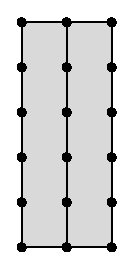
\includegraphics[height=40mm]{fregm2-1.eps}\hspace{20mm}
    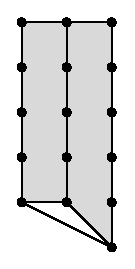
\includegraphics[height=40mm]{fregm2-2.eps}\hspace{20mm}
    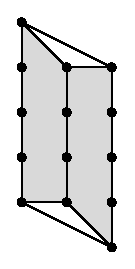
\includegraphics[height=40mm]{fregm2-3.eps}
  \end{center}
  is regular. But this can be derived from
  Lemma~\ref{lem:stripreg}.  One starts from an arbitrary
  prescribed strictly convex function on the middle column, and after
  the extensions to the two shaded vertical trapezoids of width one
  obtained from Lemma~\ref{lem:stripreg}, one adds a piecewise linear
  function that is constant on the left strip, linear on the right
  strip, and sufficiently large on the right column of vertices.
\end{proof}

Similarly, one proves the following  strengthening of
Lemma~\ref{lem:supermulreg} for $n_2=1$, as announced earlier.

\begin{lemma}
  \label{lem:patchreg1strip}
  For $m,n\geq 1$, we have
  $$
  \freg(m,n+1)\geq\freg(m,n)\cdot\binom{2n}{n}\ .
  $$
\end{lemma}



\subsection{Limit capacities}

In the following, we will show that the capacities $c(m,n)$ and
$\creg(m,n)$ (with $f(m,n)=2^{c(m,n)mn}$ and
$\freg(m,n)=2^{\creg(m,n)mn}$) asymptotically behave well, which
allows us to focus on their limits subsequently. Note that all
capacities are bounded (see Theorem~\ref{thm:anclin}).

\begin{prop}
  Let $m\geq 1$.
  \begin{enumerate}
    \item[\rm(i)] The limit \ 
       $c_m:=\displaystyle\lim_{n\rightarrow\infty}  c   (m,n)$ \ exists.
    \item[\rm(ii)] The limit \ 
   $\creg_m:=\displaystyle\lim_{n\rightarrow\infty} \creg(m,n)$ \ exists.
  \end{enumerate}
\end{prop}

\begin{proof}
  Lemmas~\ref{lem:supermul}(i) and~\ref{lem:supermulreg} imply by
  Fekete's lemma \cite[Lemma 11.6]{LW} that
  $$
  \lim_{n\rightarrow\infty}f(m,n)^{\frac{1}{n}}
  \qquad\text{and}\qquad
  \lim_{n\rightarrow\infty}\freg(m,n-1)^{\frac{1}{n}}  
  $$
  exist. Therefore,  
  $$
    \lim_{n\rightarrow\infty}\frac{1}{m}\log f(m,n)^{\frac{1}{n}}
   =\lim_{n\rightarrow\infty}\frac{\log f(m,n)}{mn}
   =\lim_{n\rightarrow\infty}c(m,n)
  $$
  and
  $$
    \lim_{n\rightarrow\infty}\frac{n}{m(n-1)}\log \freg(m,n-1)^{\frac{1}{n}}
   =\lim_{n\rightarrow\infty}\frac{\log \freg(m,n-1)}{m(n-1)}
   =\lim_{n\rightarrow\infty}\creg(m,n)
   $$
  exist as well.
\end{proof}

While the last proposition concerned the asymptotics of growing~$n$ for
fixed~$m$, the next result shows that also growing~$m$ and~$n$
simultaneously yields nice asymptotics.


\begin{prop}
  Let $m\geq 1$.
  \begin{enumerate}
  \item[\rm(i)] The limit
    $c:=\displaystyle\lim_{m\rightarrow\infty}c(m,m)$ exists. It
    satisfies
    $$
    c=\displaystyle\lim_{m\rightarrow\infty}c_m
    \qquad\text{and}\qquad
    c_{m_0}\leq c\quad (m_0\in\N)\ .
    $$
  \item[\rm(ii)] The limit
    $\creg:=\displaystyle\lim_{m\rightarrow\infty}\creg(m,m)$
    exists. It satisfies
    $$
    \creg=\displaystyle\lim_{m\rightarrow\infty}\creg_m
    \qquad\text{and}\qquad
    \creg_{m_0}\leq \creg\quad (m_0\in\N)\ .
    $$

  \end{enumerate}
\end{prop}

\begin{proof}
  From Lemma~\ref{lem:supermul}(i) one derives (for $m_0,n_0\geq 1$)
  the inequality
  \begin{equation}
    \label{eq:diaglim1}
    f(m,n)\geq f(m_0,n_0)^{\lfloor\frac{m}{m_0}\rfloor\lfloor\frac{n}{n_0}\rfloor}.
  \end{equation}
  For integers $p,q\geq 1$ we define $\Phi(p,q):=1-\frac{p\mod q}{p}$. We have
  $\Phi(q,q)=1$ and $\lim_{p\rightarrow\infty}\Phi(p,q)=1$ for all
  $q\in\N$. 

  Equation(\ref{eq:diaglim1}) then implies
  \begin{equation}
    \label{eq:diaglim2}
    c(m,n)\geq\Phi(m,m_0)\Phi(n,n_0)c(m_0,n_0)\ ,
  \end{equation}
  and, in particular,
  \begin{equation}
    \label{eq:diaglim3}
    c(m_0,n)\geq\Phi(n,n_0)c(m_0,n_0)\ .
  \end{equation}
  Inequality~(\ref{eq:diaglim3}) (together with
  $\displaystyle\lim_{n\rightarrow\infty}\Phi(n,n_0)=1$) yields
  \begin{equation}
    \label{eq:diaglim4}
    c_m\geq c(m,n_0)\ .
  \end{equation}
  Inequality~(\ref{eq:diaglim2}) implies (together
  with $\displaystyle\lim_{m\rightarrow\infty}\Phi(m,m_0)\Phi(m,n_0)=1$)
  $$
  \liminf_{m\rightarrow\infty} c(m,m)\geq c(m_0,n_0)\ ,
  $$
  and therefore,
  \begin{equation}
    \label{eq:diaglim5}
    \liminf_{m\rightarrow\infty} c(m,m)\geq c_{m_0}\ .
  \end{equation}
  
  Finally, we obtain the following chain of inequalities, which, 
  together with (\ref{eq:diaglim5}) proves part~(i) of the proposition.
  The middle inequality is from~(\ref{eq:diaglim5}), and the
  outer ones are due to~(\ref{eq:diaglim4}).
  $$
          \liminf_{m\rightarrow\infty}c_m
    \geq  \liminf_{m\rightarrow\infty}c(m,m)
    \geq  \limsup_{m\rightarrow\infty}c_m
    \geq  \limsup_{m\rightarrow\infty}c(m,m)
  $$

  Part~(ii) is proved similarly, starting from Lemma~\ref{lem:supermulreg}.
\end{proof}

Note that a similar proof yields
$$
c=\lim_{m\rightarrow\infty}c(\alpha m,\beta n)
\qquad\text{and}\qquad
\creg=\lim_{m\rightarrow\infty}\creg(\alpha m,\beta n)
$$
for each pair $\alpha,\beta>0$.

By Lemma~\ref{lem:supermul}(ii), the corresponding ``irregular limit
capacities'' do exist as well, and they are equal to $c_m$
($m\ge3$) and $c$, respectively. Therefore, we do not treat them
explicitly.





\subsection{Lower bounds}\label{subsec:lower_bounds}


\begin{prop}
  The following estimates hold.
  \begin{enumerate}
    \item[\rm(i)] $c_1=\creg_1=2$
    \item[\rm(ii)] $c_2=\creg_2>2.044$
    \item[\rm(iii)] $c_3>2.051$, $c_4>2.055$
    \item[\rm(iv)] $c_m>2.048$ for $m\geq 5$
    \item[\rm(v)] $c_m\ge\creg_m>2$ for $m\geq 3$
  \end{enumerate}
\end{prop}

\begin{proof}
  Part~(i) follows from 
  $$
  f(1,n)=\freg(1,n)=\binom{2n}{n}\approx\frac{2^{2n}}{\sqrt{2n}}\ .
  $$
  Parts~(ii) and~(iii) are results of the computer calculations
  reported in Section~\ref{sec:values}, combined with
  Proposition~\ref{prop:fregm12}(ii).

  Lemma~\ref{lem:supermul}(i) applied to the ``transposed grids'' implies 
  \begin{equation}
    \label{eq:lowerbounds}
    c(m_1+m_2,n)\geq\frac{m_1}{m_1+m_2}c(m_1,n)+\frac{m_2}{m_1+m_2}c(m_2,n)\ ,    
  \end{equation}
  and thus 
  $$
  c_{m_1+m_2}\geq\frac{m_1}{m_1+m_2}c_{m_1}+\frac{m_2}{m_1+m_2}c_{m_2}\ .
  $$
  With~(ii) and~(iii), this yields~(iv).

  Similarly, Lemma~\ref{lem:patchreg1strip} leads to
  $$
  \creg_{m+1}\geq \frac{m}{m+1}\creg_m+\frac{1}{m+1}\cdot 2\ .
  $$
  With~(ii) this proves part~(v).
\end{proof}

Equation~(\ref{eq:lowerbounds}) implies that $c_{kn}\ge c_n$ for
$k\ge2$; for example, this implies that $c_4\ge c_2$ --- but it is not
obvious that $c_3\ge c_2$. Even stronger, one would assume that
\[
2 = c_1 <  c_2 <  c_3 < \ \cdots\ \ \le c\ ,
\]
and
\[
2 = \creg_1 <  \creg_2 <  \creg_3 < \ \cdots\ \ \le \creg\ ,
\]
but neither monotonicity is proved.


\subsection{Upper bounds}\label{subsec:upper_bounds}

From general principles (see Ajtai et al. \cite{ACNS}) one
gets that the capacity for any configuration of $N$ points in the plane
is finite. In the general position case (no three points on a line)
the currently best upper bound is $o(2^{59N})$,
due to Santos \& Seidel \cite{SantosSeidel}.
However, in the very ``degenerate'' case of lattice triangulations,
there are far fewer triangulations:
Orevkov \cite{Orevkov} obtained the bound $f(m,n)\le4^{3mn}=2^{6mn}$.
Very recently, this has been substantially improved by
Anclin \cite{Anclin}, as follows.

\begin{theorem}[Anclin \cite{Anclin}]
\label{thm:anclin}
For all $m,n\ge1$,
\[
f(m,n)\ <\ 2^{3mn-m-n}.
\] 
\end{theorem}

\begin{proof}
Our sketch relies on the essential ideas of Anclin's proof.

The first, crucial observation is that the
midpoints of the edges in any unimodular triangulation 
are exactly the half-integral, not integral points
in~$\conv(P_{m,n})$. (Clearly the midpoint of every edge
is half-integral; the converse
may be derived from Pick's theorem, or from the fact that all 
unimodular triangles are
equivalent to~$\conv\{(0,0),(1,0),(0,1)\}$.)
The number of these half-integral points in the interior of~$P_{m,n}$ 
is $e=3mn-m-n$.

Now any triangulation is built as follows:
The half-integral points are processed in 
an order that is given by a parallel \emph{sweep}.
(See de Berg et al.~\cite[Sect.~2.1]{4Marks}
for a discussion and many further sweeping applications
of this fundamental technique.)

Whenever a point is processed, we add to the partial
triangulation a new edge with the given midpoint.
The key \emph{claim} is that at each such step,
when a half-integral point $v$ is processed, 
there are (at least one and) at most two possibilities
for the new edge with midpoint $v$ to be added.
If this claim is true, then the number of triangulations
is bounded by $2^e$.
\[
\input{anclin1.pstex_t}\qquad\input{anclin2.pstex_t}
\]
To prove the claim, one can verify the following:
Let $[v',\bar v']$ and $[v'',\bar v'']$
be two potential edges with midpoint $v$ that could be added,
where $v'$ and $v''$ are the endpoints below the sweep-line $\ell$;
let $Q$ be the convex hull of the integral points in
the triangle $[v,v',v'']$; then all the $k\ge2$
vertices $v'=v_0,v_1,\dots,v_{k-1},v_k=v''$
of $Q$ are ``visible'' from $v$, and any one of the edges $[v_i,\bar v_i]$
with midpoint $v$ could potentially be added at this step.
Furthermore, the midpoints $\frac12(v_{i-1}+v_i)$ lie below
the sweep-line, and thus the edges $[v_{i-1}v_i]$
are present in the current partial triangulation.
\[
\input{anclin3.pstex_t}
\]
Now assume that $[v_0,\bar v_0]$, $[v_1,\bar v_1]$, $[v_2,\bar v_2]$
are three \emph{adjacent} edges with midpoint $v$ that could be added when
processing $v$. By central symmetry with respect to~$v$
we may assume that the midpoint $w$
of $[v_1,\bar v_2]$ lies below the sweep-line. But the
triangle $[v_1,v,\bar v_2]$ is then an empty triangle of area
$\frac14$, just like the triangle $[v_1,v,v_2]$. From this
we conclude that in the current partial triangulation, 
the edge $[v_1,\bar v_2]$ must be present --- which creates
a crossing with the potential edge $[v_0,\bar v_0]$, and thus 
a contradiction.
\end{proof}

The following upper bounds on the limit capacities follow immediately
from Theorem~\ref{thm:anclin}.

\begin{cor}
For all $m,n\ge 1$, the following inequalities hold:
\begin{enumerate}
  \item[\rm (i) ] $\creg(m,n)\ \le\ c(m,n)\ \le\ 3-\frac1m -\frac1n$
  \item[\rm (ii) ] $\creg_m\ \le\ c_m\ \le\ 3-\frac1m$ \quad 
      {\rm  (in particular, $\creg_2\le c_2\le 2.5$)}
  \item[\rm (iii) ] $\creg\ \le\ c\ \le\ 3$
\end{enumerate}
\end{cor}

As Anclin noted, his proof works much more generally:
For any partial triangulation of a not necessarily simple or convex
lattice polygon, the number of completions is at most $2^{e'}$,
where $e'$ is 
the number of edges that are to be added.

%For the case of a strip, $m=2$, we get a better upper bound as
%follows.


%\begin{prop}
%For lattice rectangles of width~$2$, one has upper bounds
%\[
%f(2,n) \ \le\ 2^n\binom{2n}{n}^2\ <\ 2^{5n},
%\]
%and hence $\creg_2=c_2 \le 2.5$.
%\end{prop}

%\begin{proof}
%In every triangulation of a $2\times n$ strip
%all the ``width~$2$ diagonals'' are flippable. Thus the triangulation
%can be encoded by a
%triangulation that decomposes into two $1\times n$ strips
%plus a collection
%of vertical middle edges that have to be flipped. This yields
%the desired bound.
%\end{proof}

%%% Local Variables:
%%% mode: latex
%%% TeX-master: "bcc_ct"
%%% End:
